\documentclass{article}
\usepackage[top=1.5cm, bottom=1.5cm, left=1.5cm, right=1.5cm]{geometry}
\usepackage[utf8]{inputenc}
\usepackage{enumitem}
\usepackage{graphicx}
\usepackage{textcomp}
\usepackage{amssymb}

\title{Facultad de Ciencias. \\Tarea 4. \\ Fundamentos de Bases de Datos.}
\author{Arteaga Hernández Alejandro Iabin \and 
        Barocio Gómez Luis Fernando }
\date{\textbf{Fecha entrega 5 de Abril de 2020}}

\begin{document}

\maketitle

\begin{enumerate}
    %%%Pregunta 1%%%
    \item Cardinalidad de la consulta
    
    Considera las siguientes relaciones: 
    
    \begin{center}
        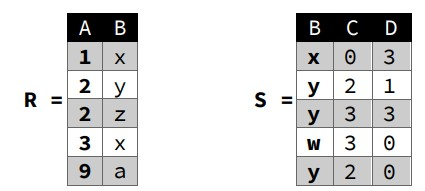
\includegraphics[scale=0.5]{p1.jpg}
    \end{center}

    Para las siguientes expresiones de \textbf{álgebra relacional}, completa la tabla con el número de tuplas que cada una de ellas produce utilizando las relaciones \textbf{R} y \textbf{S}.
   
   \begin{center}
        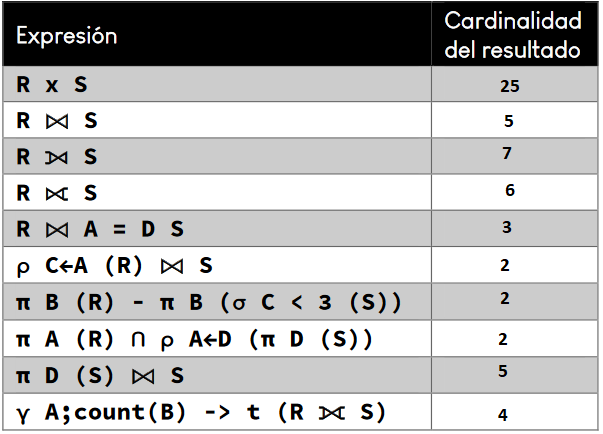
\includegraphics[scale=0.5]{0.png}
   \end{center}
    %%%Pregunta 2%%%
    \item Banco del Sur.
    
    Supón que tienes el siguiente \textbf{esquema de una base de datos} para una institución bancaria:
    
    \begin{center}
        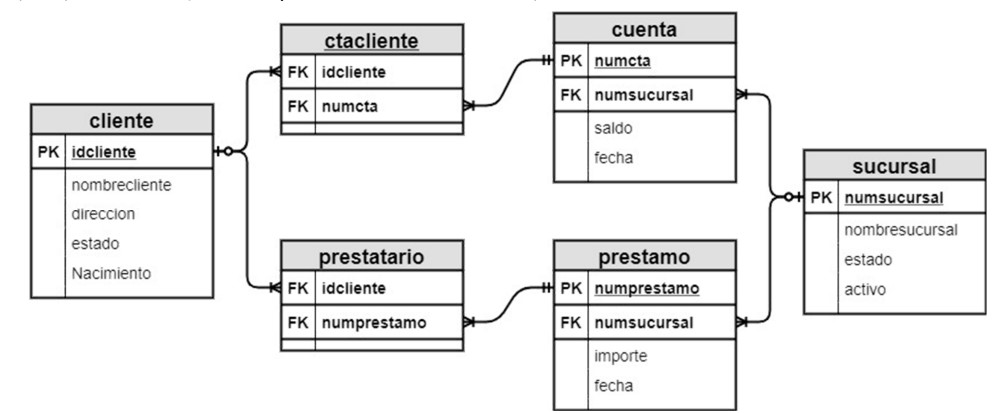
\includegraphics[scale=0.4]{p2.jpg}
    \end{center}
    
    Escribe una \textbf{expresión de álgebra relacional} para responder las siguientes consultas. Deberás comprobar cada una ellas en \textbf{Relax} y agregar en cada inciso una captura de pantalla con el resultado obtenido.
    
    \begin{enumerate}[label=\alph*)]
        \item Encontrar la información de todas las cuentas otorgadas en la sucursal \textbf{HUATULCO} durante \textbf{2015}
        
        $\pi$ numcta, numsucursal, saldo, fecha ($\sigma$ sucursal.nombresucursal = 'HUATULCO' $\land$ cuenta.fecha $\geq$ date('2015-01-01') $\land$ cuenta.fecha $<$ date('2016-01-01') (cuenta $\bowtie$ sucursal))
        
        \begin{center}

            
\includegraphics[scale=0.5]{1.jpg}
        \end{center} 
        
        \item Obtener toda la información de los clientes que viven en \textbf{CHIAPAS}, que hayan nacido en \textbf{1969} y que tengan algún préstamo. Mostrar la información \textbf{ordenada} por el nombre del cliente.
    
        $\tau$ nombrecliente $\pi$ idcliente, nombrecliente, direccion, estado, nacimiento ($\sigma$ estado = 'CHIAPAS' $\land$ nacimiento $\geq$ date('1969-01-01') $\land$ nacimiento $<$ date('1970-01-01') cliente $\bowtie$ prestatario)
        
        \begin{center}
            
\includegraphics[scale=0.5]{2.jpg}
        \end{center} 
        
        \item Toda la información de los clientes del banco que tiene una cuenta, un préstamo o ambas y que vivan en \textbf{CHIAPAS}.
        
        $\pi\ idcliente,\ nombrecliente,\ direccion,\ estado,\ nacimiento\ (\sigma\ numprestamo \neq null \lor numcta \neq null\ (\sigma\ estado = 'CHIAPAS'\ (cliente \bowtie prestatario \bowtie ctacliente)))$
        
        \begin{center}
            
\includegraphics[scale=0.5]{3.jpg}
        \end{center} 
        
        \item Relación de los clientes que \textbf{tienen un crédito} con importe mayor o igual a \textbf{\$80,000.00} pero \textbf{no tienen ninguna cuenta en el banco}. Mostrar el \textbf{idcliente, nombre del cliente, número de préstamo e importe}
        
        $\pi\ idcliente,\ nombrecliente,\ numprestamo,\ importe\ (\sigma\ importe \geq 80000 \land numcta = null\ (cliente \bowtie prestatario \bowtie prestamo \bowtie ctacliente))$
        
        \begin{center}
            
\includegraphics[scale=0.5]{4.jpg}
        \end{center} 
        
        \item Todos los clientes que \textbf{tienen un préstamo y una cuenta}, que hayan nacido en \textbf{YUCATÁN o CAMPECHE.}
        
        $\sigma$ estado = 'YUCATÁN' $\lor$ estado = 'CAMPECHE' cliente $\bowtie$ prestatario $\bowtie$ ctacliente
        
        \begin{center}
            
\includegraphics[scale=0.5]{5.jpg}
        \end{center} 
        
        \item Información de los clientes que hayan nacido en \textbf{YUCATÁN} que tienen un crédito en la sucursal \textbf{QUINTANA ROO.}
        
        $\pi$ idcliente, nombrecliente, direccion, estado, nacimiento ($\sigma$ estado = 'YUCATÁN' $\land$ estadosucursal = 'QUINTANA ROO' (cliente $\bowtie$ prestatario $\bowtie$ prestamo $\bowtie$ $\rho$ estadosucursal$\leftarrow$ estado sucursal))
        
        \begin{center}
            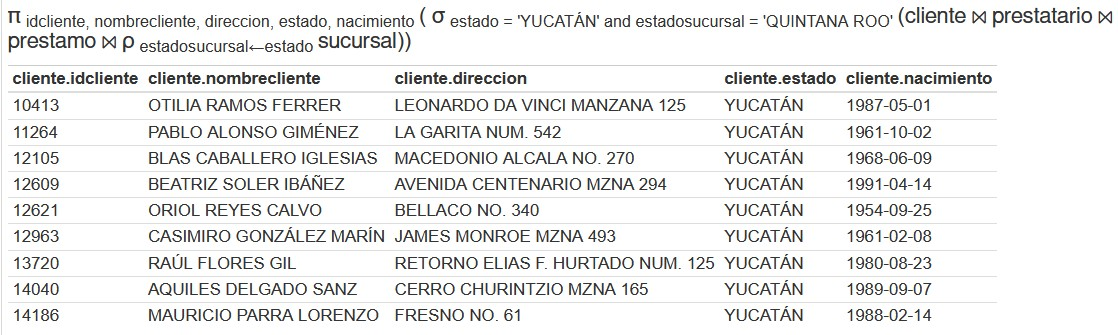
\includegraphics[scale=0.5]{6.jpg}
        \end{center} 
        
        \item Nombre de todos los clientes que tienen \textbf{un préstamo} y \textbf{el importe} del mismo. El importe debe ser de entre \textbf{\$50,000} y \textbf{\$80,000}, el préstamo se debió entregar durante el mes de \textbf{febrero de 2014}
        
        $\pi$ nombrecliente, importe ($\sigma$ importe $\geq$ 50000 $\land$ importe $\leq$ 80000 $\land$ fecha $\geq$ date('2014-02-01') $\land$ fecha $<$ date('2014-03-01') (cliente $\bowtie$ prestatario $\bowtie$ prestamo))
        
        \begin{center}
            
\includegraphics[scale=0.5]{7.jpg}
        \end{center} 
        
        \item Toda la información de las sucursales con clientes que tengan una cuenta abierta en el banco otorgada en el estado de \textbf{GUERRERO} y que viven en \textbf{GUERRERO}.
        
    $\pi$ numsucursal, nombresucursal, estado, activo ($\sigma$ estado = 'GUERRERO' $\land$ estadosucursal = 'GUERRERO' (cliente $\bowtie$ ctacliente $\bowtie$ cuenta $\bowtie$ $\rho$ estadosucursal$\leftarrow$ estado (sucursal)))
        
        \begin{center}
            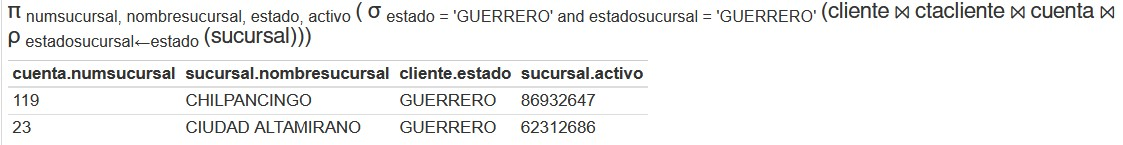
\includegraphics[scale=0.5]{8.jpg}
        \end{center} 
        
        \item Toda la información de los clientes que tienen solo cuenta y aquellos que tienen solo préstamo en el banco.
        
        $\pi\ idcliente,\ nombrecliente,\ direccion,\ estado,\ nacimiento\ \sigma\ numprestamo \neq null\ xor\ numcta \neq null\ (cliente \bowtie prestatario \bowtie ctacliente)$
        
        \begin{center}
            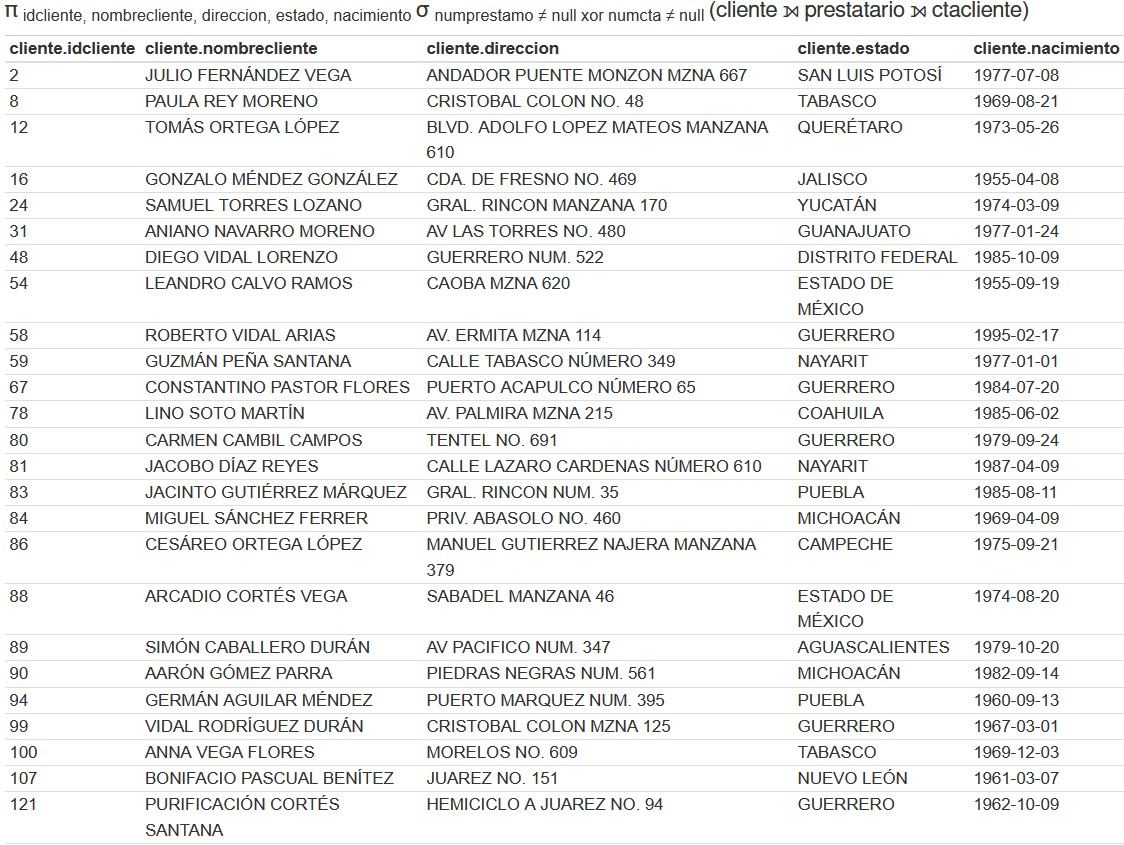
\includegraphics[scale=0.5]{9.jpg}
        \end{center} 
        
        \item Una lista que muestre el estado, el nombre de sucursal y total de clientes que se tienen, considerando que los clientes deben tener cuenta con saldo mayor a \textbf{\$60,000.00}.
        \begin{center}
            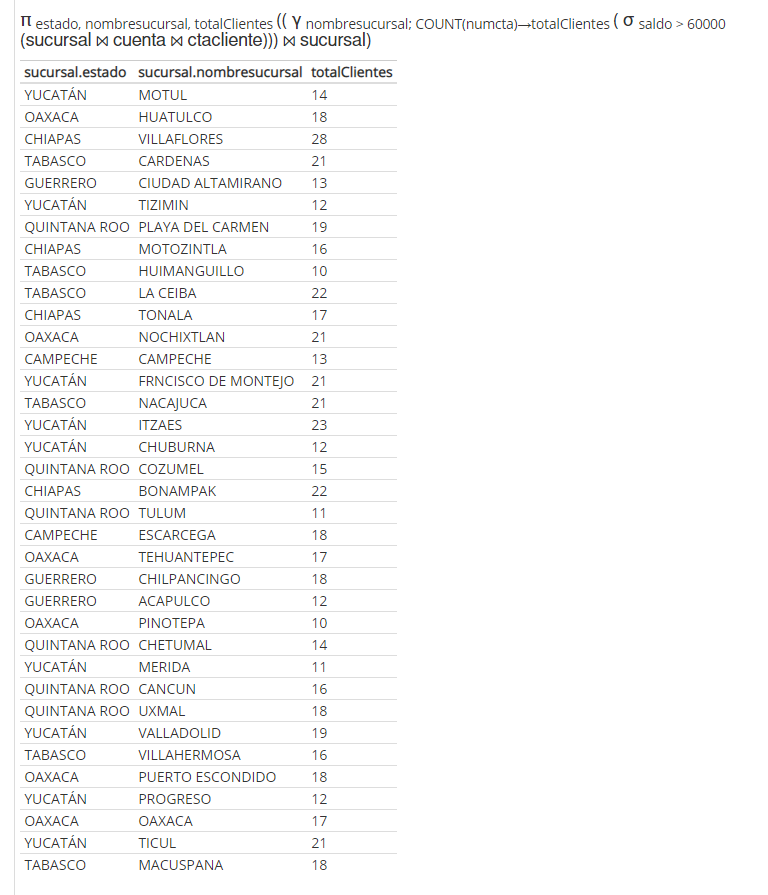
\includegraphics[scale=0.5]{2j.PNG}
        \end{center} 
        
        \item Información de los clientes con saldo entre \textbf{\$15,000.00} y \textbf{\$30,000.00} que no han solicitado préstamos.
                \begin{center}
            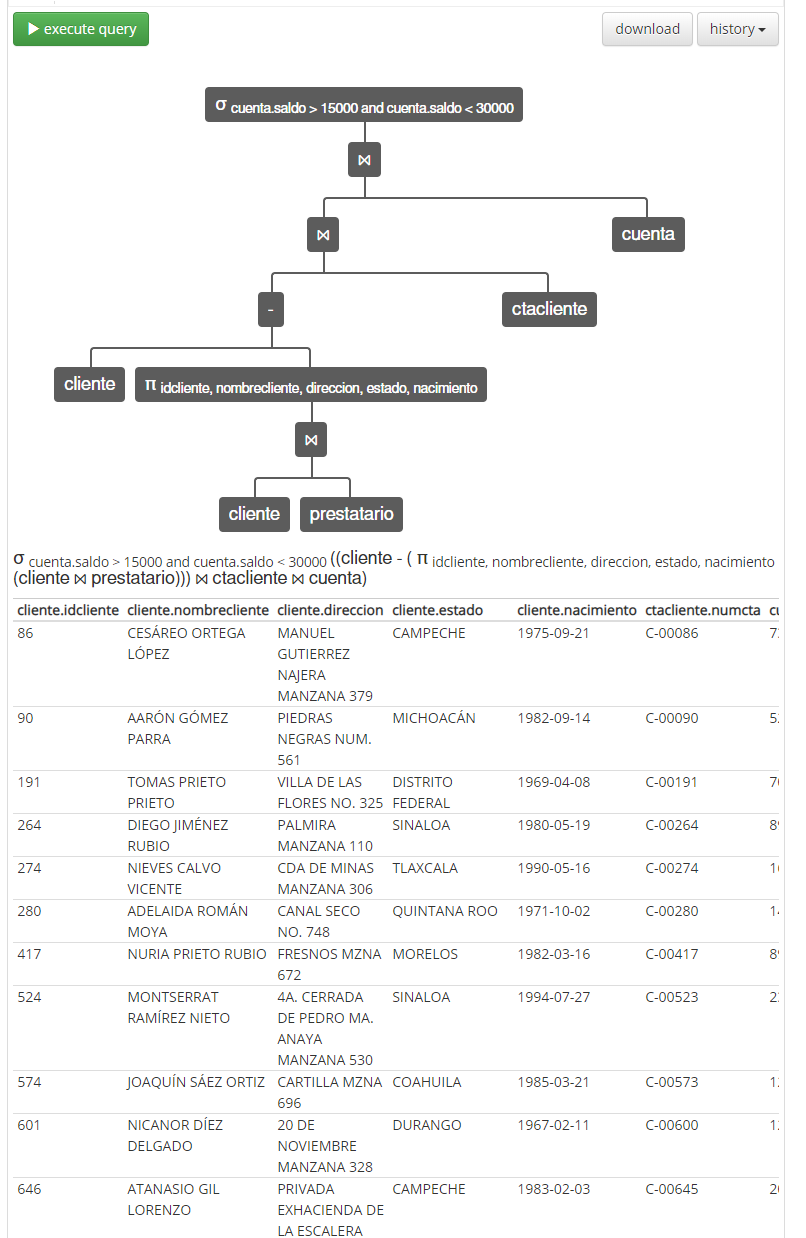
\includegraphics[scale=0.5]{2k.PNG}
        \end{center} 
        
        \item Una lista con el \textbf{saldo promedio, mayor saldo, menor saldo, y total de cuentas}, por estado y sucursal. El saldo promedio debe ser mayor que \textbf{\$85,000.00}
                \begin{center}
            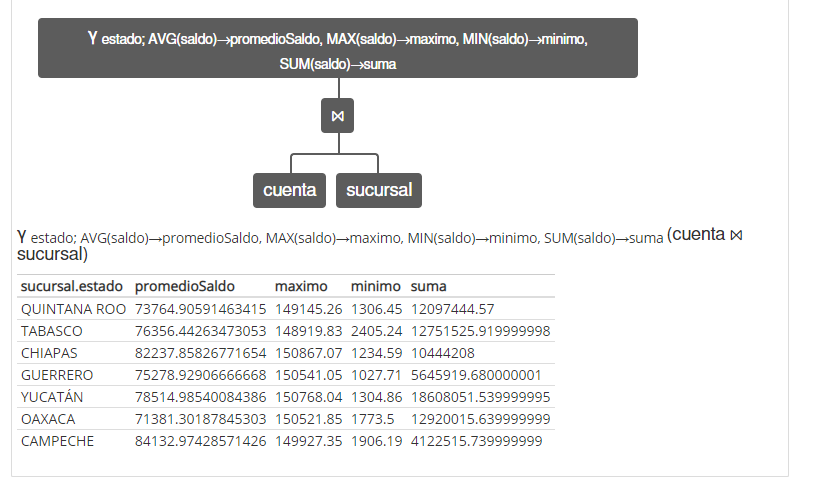
\includegraphics[scale=0.5]{2la.PNG}
        \end{center} 
                \begin{center}
            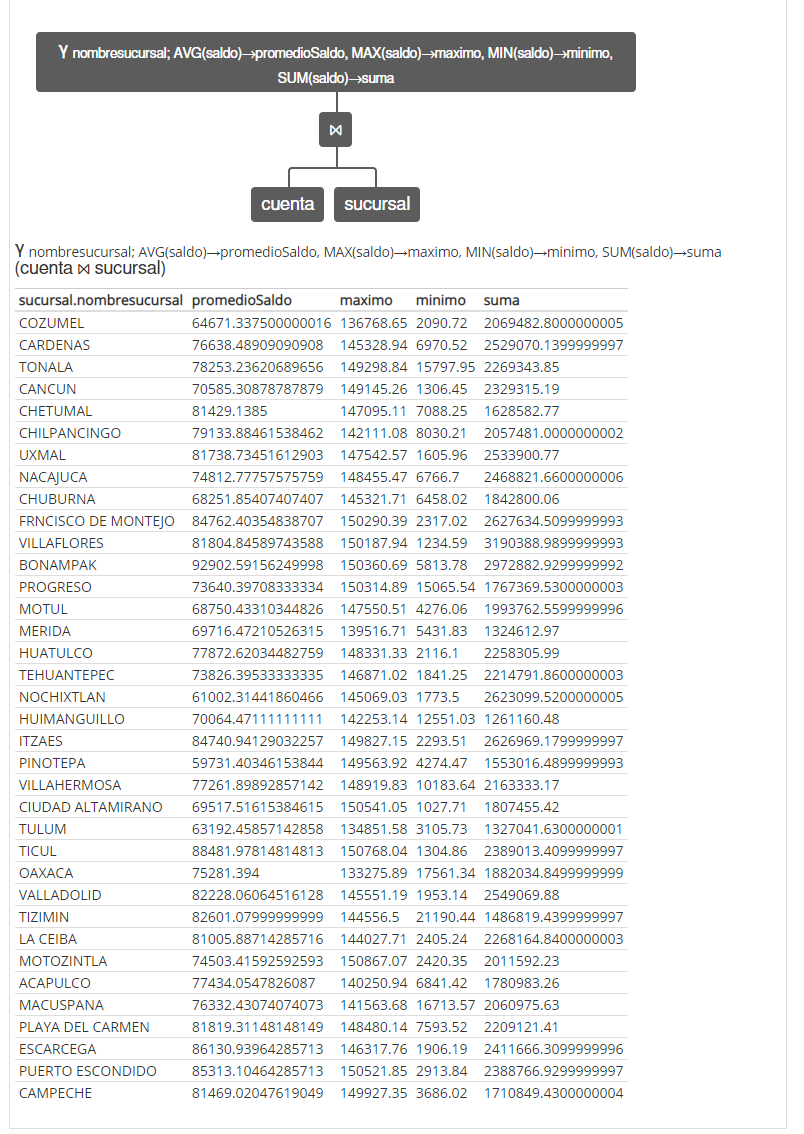
\includegraphics[scale=0.5]{2lb.PNG}
        \end{center} 
        \item El estado que ha otorgado la \textbf{mayor cantidad de préstamos}, cuyo importe esté entre \textbf{\$100,000.00} y \textbf{\$120,000.00}. Se debe mostrar también el total de préstamos. 
                \begin{center}
            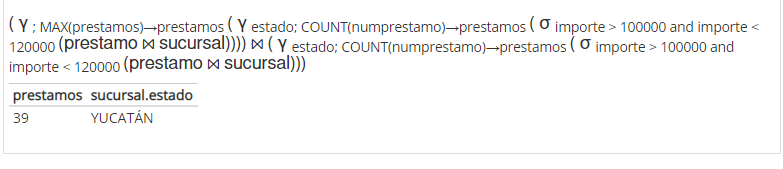
\includegraphics[scale=0.5]{2m.PNG}
        \end{center} 
        
        \item El \textbf{id, nombre del cliente, sucursal y saldo} de aquel cliente que tenga el menor saldo de todas las cuentas del banco.
        
                \begin{center}
            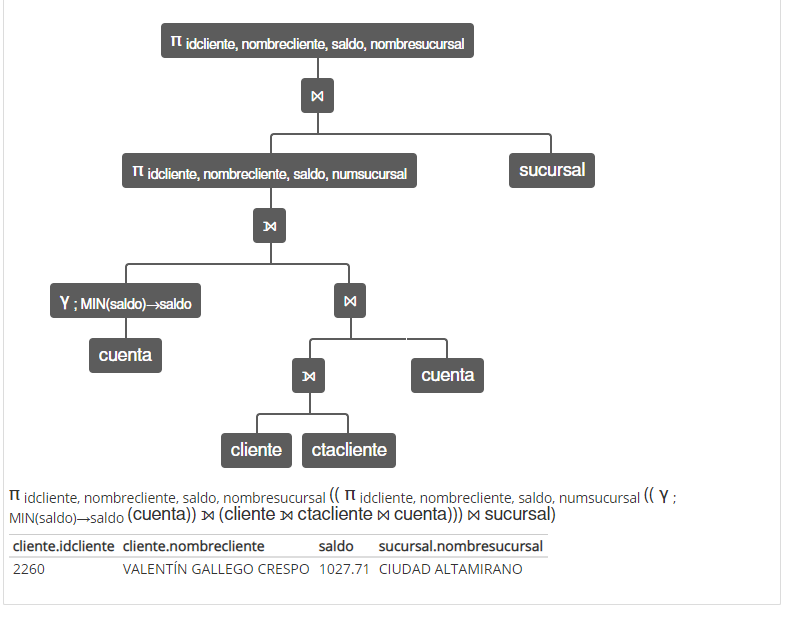
\includegraphics[scale=0.5]{2n.PNG}
        \end{center} 
        \item El \textbf{nombre de la sucursal} y el \textbf{saldo promedio}, de aquella que tiene el menor saldo promedio de todas las sucursales del banco.
                \begin{center}
            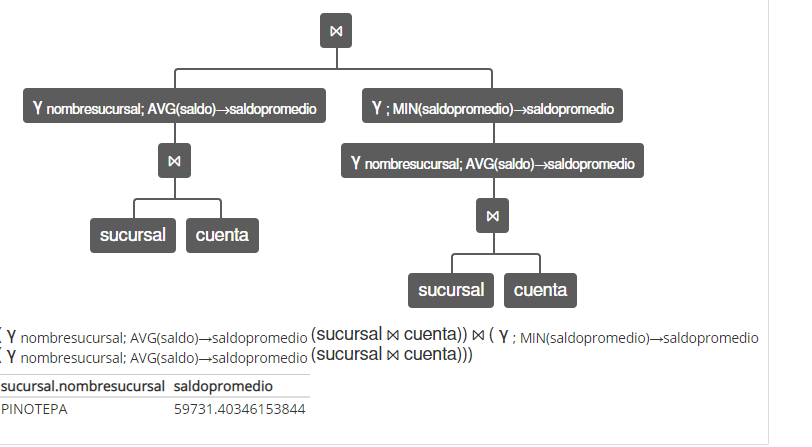
\includegraphics[scale=0.5]{2o.PNG}
        \end{center} 
        
    \end{enumerate}
    
    \textbf{Operaciones de mantenimiento de datos: borrado, inserción y actualización.}
    \textbf{EN LAS PRIMERAS 3 RESPUESTAS SOLO FALTA AGREGAR LA PARTE DE REINSERTAR ESA RELACIÓN 
    R <- R'}
    \begin{enumerate}[label=\alph*)]
        \item Borrar toda la información de cuentas del \textbf{EDMUNDO RUBIO MONTERO.}
           \begin{center}
            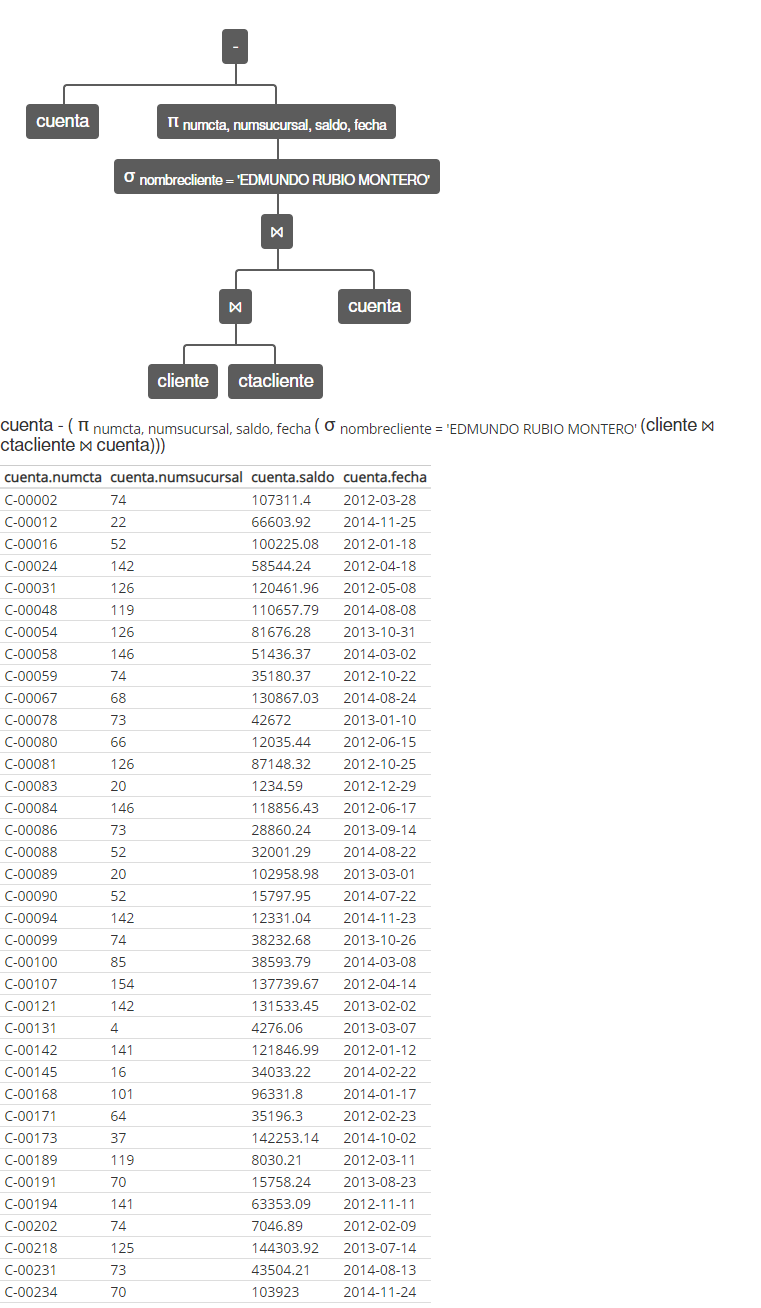
\includegraphics[scale=0.5]{3a.PNG}
        \end{center}
        \item Borrar todas las cuentas de la sucursal \textbf{CHILPANCINGO}.
          \begin{center}
            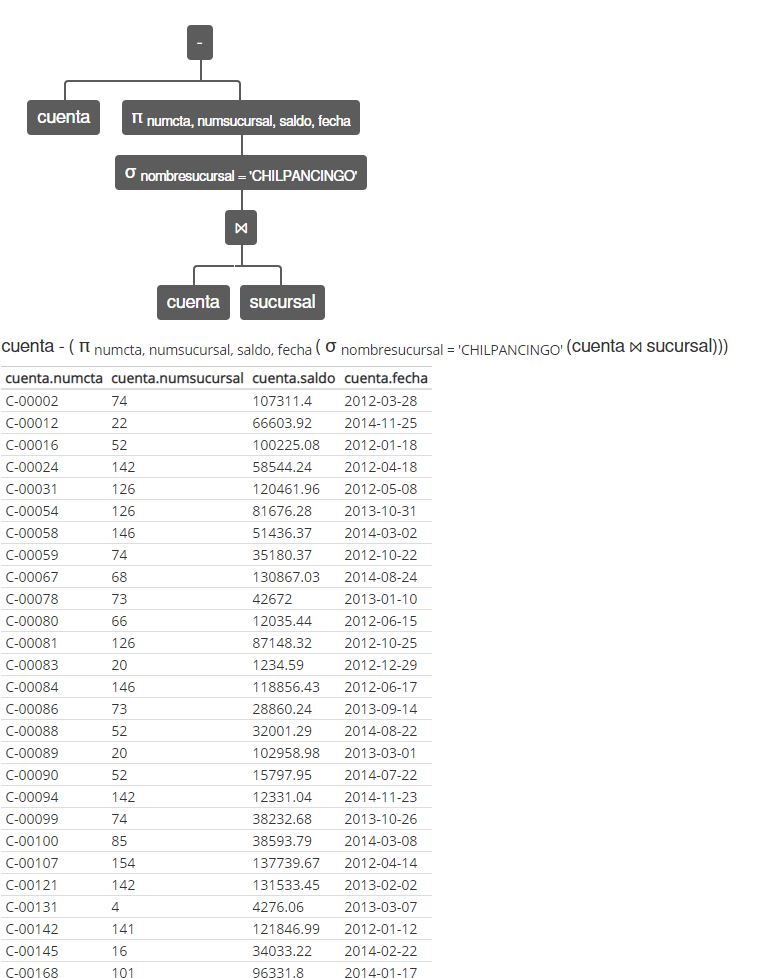
\includegraphics[scale=0.5]{3b.PNG}
        \end{center}
        \item Borrar la información de los préstamos otorgados durante \textbf{2015}.
          \begin{center}
            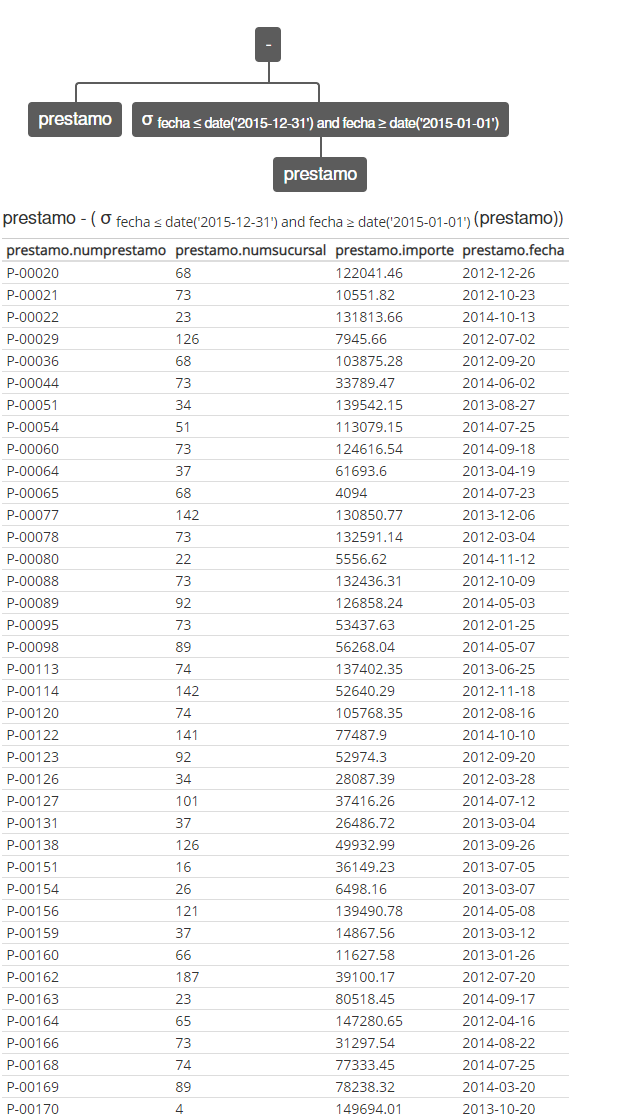
\includegraphics[scale=0.5]{3c.PNG}
        \end{center}
        
        \textbf{EN ESTA PARTE AGREGAR LA ELIMINACIÓN QUE ANTECEDE A LA NUEVA INSERCIÓN 
        PARA QUE SEA UPDATE, SOLO SE PUSO LA PARTE DE LA INSERCION POR CLARIDAD, PERO INSERTAR LA ELIMINACIÓN TAMBIEN}
        \item Otorgar el préstamo \textbf{P-05293} a la clienta \textbf{ELISA NIETO FERRER} con importe de \textbf{\$50,000}. El préstamo se otorgará en la misma sucursal donde tiene dada de alta su cuenta.
            \begin{center}
            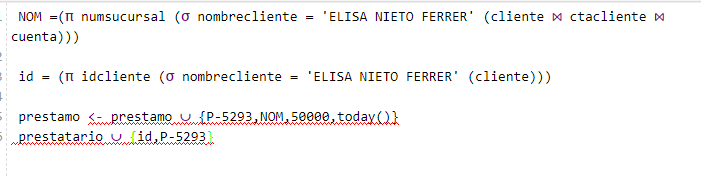
\includegraphics[scale=0.5]{3d.PNG}
        \end{center}
        \item Ofrecer un nuevo préstamo con \textbf{\$20,000.00} a todos los clientes que tienen cuenta con saldo mayor de \textbf{\$80,000.00} en la sucursal \textbf{BONAMPAK}, el número de préstamo será el de la nueva cuenta. Si el saldo es menor o igual a \textbf{\$80,000.00}, se les otorgará un préstamo de \textbf{\$15,000.00}
        
        \item Aumentar el importe del préstamo \textbf{P-00197} de \textbf{JACOBO PARRA ORTEGA} en un \textbf{15\%}.
            \begin{center}
            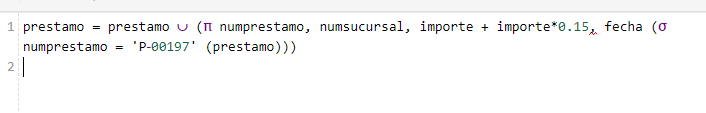
\includegraphics[scale=0.5]{3f.PNG}
        \end{center}
        \item Aumentar todos los saldos de la sucursal \textbf{CARDENAS} en un \textbf{8\%}
            \begin{center}
            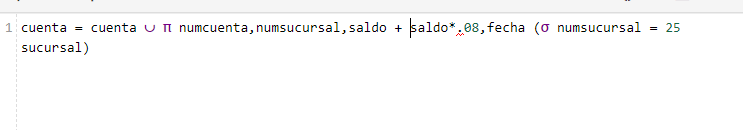
\includegraphics[scale=0.5]{3g.PNG}
        \end{center}
        \item Disminuir \textbf{8\%} a las cuentas con saldo mayor a \textbf{\$90,000} y a las demás en un \textbf{4\%}. Las cuentas deben estar ubicadas en la sucursal \textbf{HUATULCO}.
            \begin{center}
            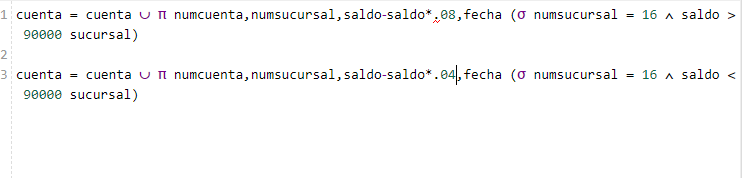
\includegraphics[scale=0.5]{3h.PNG}
        \end{center}
        
    \end{enumerate}
    
\end{enumerate}

\end{document}
